\documentclass[12pt, letterpaper]{article}
\usepackage[margin=1in]{geometry}
\usepackage{amsmath,amsthm,array, amssymb,amsfonts, enumitem, fancyhdr, color, comment, graphicx, environ}

\author{Val Anthony Balagon}
\date{January 2019}
\title{Chapter 4: Orthogonality}

%User commands
\newcommand{\R}[1]{$\mathbb{R}^{#1}$}
\newcommand{\Vector}[1]{$\textbf{#1}$}
\newcommand{\V}[1]{\textbf{\textit{#1}}}

\newcommand{\A}{$A$}
\newcommand{\x}{\textbf{\textit{x}}}
\newcommand{\B}{\textbf{\textit{b}}}
\newcommand{\system}{\textbf{\textit{\A \x = \B}}}
\newcommand{\nullsystem}{\textbf{\textit{\A\x}} = \textbf{0}}
\newcommand{\DefinitionSpace}{\vspace{15px}}


\newtheorem*{remark}{Remark}
\theoremstyle{definition}
\newtheorem{definition}{Definition}[section]
\newtheorem{example}{Example}


\newcommand*{\vertbar}{\rule[-1ex]{0.5pt}{2.5ex}}



\begin{document}
	\maketitle
	\begin{abstract}
		This chapter focuses on the orthogonality of the four subspaces, projections, and least squares approximations.
	\end{abstract}


	Two vectors are orthogonal when their dot product is zero $\V{v} \cdot \V{w} = \V{v}^T \V{w} = 0$. This chapter will revolve around orthogonal subspaces, orthogonal bases, and orthogonal matrices.
	
	\DefinitionSpace
	\begin{definition}
		Orthogonal vectors have the following properties:
		\renewcommand{\theenumi}{\roman{enumi}}
		
		\begin{enumerate}[leftmargin=2\parindent]
			\item $\V{v}^T \V{w} = 0$
			\item $||\V{v}||^2 + ||\V{w}||^2 = ||\V{v} + \V{w}||^2$
		\end{enumerate}	
	
	\end{definition} 	

	\DefinitionSpace
	\begin{remark}
		The subspaces have orthogonal properties. 
		\begin{enumerate}
			\item \textbf{The rowspace $C(A^T)$ is perpendicular to the nullspace $N(A)$}. Every row of $A$ is perpendicular to the solution of $A\V{x} = \textbf{0}$.
			\item \textbf{The column space $C(A)$ is perpendicular to the left nullspaces $N(A^T)$}. When $\V{b}$ is outside of the column space when we're trying to solve for $A\V{x} = \V{b}$, then this nullspace of $A^T$ comes into its own. It contains the error $\V{e} = \V{b} - A\V{x}$ in the least-squares solution.
		\end{enumerate}
	\end{remark}
	\DefinitionSpace
	
	\begin{figure}[h!]
		\centering
		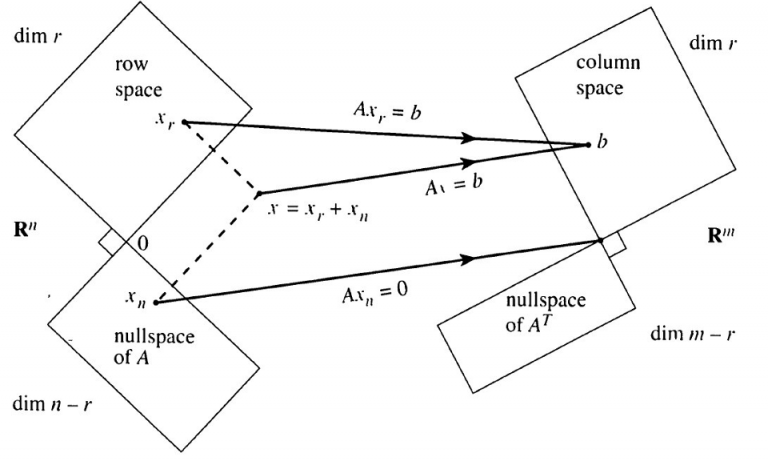
\includegraphics[scale=0.4]{4-subspaces.png}
		\caption{The Four Subspaces. There are two pairs of orthogonal subspaces.}
	\end{figure}
	

	\begin{definition}
		Two subspaces \V{V} and \V{W} of a vector space are orthogonal if every vector \V{v} in \V{V} is perpendicular to every vector \V{w} in \V{W}.
		\renewcommand{\theenumi}{\roman{enumi}}
		
		\begin{equation*}
			\V{v}^T \V{w} = 0 \text{for all \V{v} in \V{V} and all \V{w} in \V{W}.}
		\end{equation*}
	\end{definition} 	
	\DefinitionSpace
	
	
	\begin{remark}
	Every vector \V{x} in the nullspace is perpendicular to every row of $A$, because $A\V{x} = \textbf{0}$. The nullspace $N(A)$ and the row space $C(A^T)$ are orthogonal subspaces of \R{n}.
	
		\begin{equation*}
			A \V{x} = \begin{bmatrix} \text{row 1} \\ \vdots \\ \text{row m} \end{bmatrix} \begin{bmatrix} x_1 \\ \vdots \\ x_n \end{bmatrix} = \begin{bmatrix} 0 \\ \vdots \\ 0 \end{bmatrix}
		\end{equation*}
	\end{remark}
	\noindent (row 1) $\cdot \V{x}$ is zero and (row $m) \cdot \V{x}$ is also zero. Every row has a zero dot product with \V{x}. Then \V{x} is perpendicular to every combination of the rows. \textbf{The whole row space $C(A^T)$ is orthogonal to $N(A)$. }
	\DefinitionSpace
	
	
	



\end{document}